% ============================================================
% 分片：s06  对应原文 PDF 第 69--71 页
% 负责章节：B.3 末段（基态与 $\bar Q$-上同调）；B.4 A-type quantum mechanics and Morse cohomology；
%           B.5 The Morse–Smale–Witten complex
% 译者：translator-08   审校状态：初稿
% ============================================================
% ==== 原文 PDF 第 69 页 ====
% [跨页接续: 原文第68页/69页，本句接在第 68 页末式 (B.13) 之后]
现在我们证明，可以把基态等同于 $\bar Q$-上同调类。

首先，由于 $\bar Q$ 与 $H$ 对易，可以把 $\mathcal{H}$ 分解为 $H$ 的本征空间，其中 $\mathcal{H}^E$ 是能量为 $E$ 的本征空间：
\begin{equation}
  \tag{B.14}
  H(\mathcal{H},\bar Q)=\bigoplus_{E\geq0}H(\mathcal{H}^E,\bar Q|_{\mathcal{H}^E}).
\end{equation}
% [Tutor Note: 式 (B.14) 的直和分解依赖于 $\bar Q$ 保持每个能量本征空间（$\bar Q$ 与 $H$ 对易），并默认能谱离散；若谱为连续谱，则 $\bigoplus$ 应换成直积分。局域化模型的能谱在此意义上离散，故可逐本征值分块计算上同调。]
设 $|\psi\rangle$ 是能量 $E>0$ 的 $\bar Q$-闭态。可以如下构造一个态 $|\psi'\rangle$，实现 $|\psi\rangle$ 的 $\bar Q$-恰当性：
\begin{equation}
  \tag{B.15}
  |\psi'\rangle=\frac{1}{2E}Q|\psi\rangle\Rightarrow\bar Q|\psi'\rangle=\frac{1}{2E}[\bar Q,Q]|\psi\rangle=|\psi\rangle
\end{equation}
% [Tutor Note: 中间一步用到 B.3 节的关系 $[\bar Q,Q]=Q\bar Q+\bar QQ=2H$，于是 $\bar Q|\psi'\rangle=\frac{1}{E}H|\psi\rangle=|\psi\rangle$。要点在于分母恰为 $2E$：能量 $E>0$ 时该构造有效，而 $E=0$ 时 $H(\mathcal{H}^0,\bar Q|_{\mathcal{H}^0})=\mathcal{H}^0$ 反而说明零能态全部是上同调类。]
因此，每个能量为正的 $\bar Q$-闭态都必然是 $\bar Q$-恰当的，即 $H(\mathcal{H}^E,\bar Q|_{\mathcal{H}^E})=0$。另一方面，由上面的幺正性界，能量为 $0$ 的态必然是 $\bar Q$-闭的，$\bar Q|_{\mathcal{H}^0}=0$。特别地，任何 $\bar Q$-恰当的零能向量必然就是零向量：$H(\mathcal{H}^0,\bar Q|_{\mathcal{H}^0})=\mathcal{H}^0$。正如所断言，我们看到基态被等同于 $\bar Q$-上同调类：
\begin{equation}
  \tag{B.16}
  \mathcal{H}^0\cong H(\mathcal{H},\bar Q).
\end{equation}

我们常常能够给理论赋予更多的结构。例如，会有一个守恒荷 $R$，$[R,H]=0$，使得 $Q$ 的荷为 $1$、$\bar Q$ 的荷为 $-1$。若 $R$ 的荷取整数值，可以将它解释为理论的 $U(1)_R$ $R$ 对称性的生成元；于是可以按 $R$ 荷（的负值）给 Hilbert 空间 $\mathcal{H}$ 一个 $\mathbb{Z}$-分次：
\begin{equation}
  \tag{B.17}
  \mathcal{H}=\bigoplus\mathcal{H}^n,\qquad R|\psi\rangle=in|\psi\rangle,\quad|\psi\rangle\in\mathcal{H}^n.
\end{equation}
由此，$\bar Q$ 与 $Q$ 在这个 $\mathbb{Z}$-分次向量空间上的作用如下：
\begin{equation}
  \tag{B.18}
  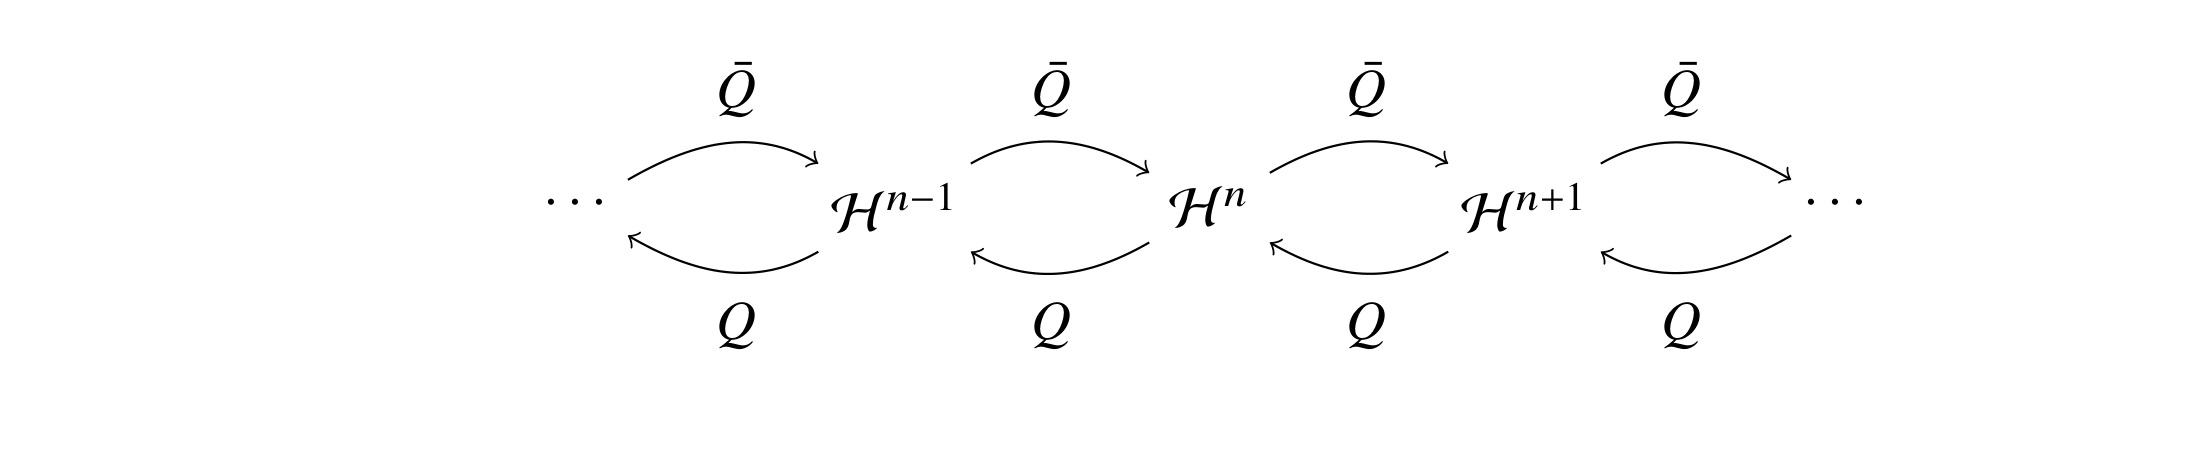
\includegraphics[width=\linewidth]{figures/inline/eq-p69-a.png}% [说明: 该式为原文矢量阶梯图，按原图无损嵌入]
\end{equation}
% [Tutor Note: 阶梯图中 $\bar Q$ 的弧箭头向右（$\mathcal{H}^{n-1}\to\mathcal{H}^n$，升度），$Q$ 的弧箭头向左（降度），$Q=\bar Q^\dagger$；这与 $R$ 荷约定（按 $R$ 荷的负值分次，$n=-R$，$\bar Q$ 的 $R$ 荷为 $-1$）以及 (B.19) 的 $H^n:=\operatorname{Ker}\bar Q|_{\mathcal{H}^n}/\operatorname{Im}\bar Q|_{\mathcal{H}^{n-1}}$ 一致。核对符号时勿把 $Q$ 当成上链微分。]
我们把 $\mathbb{Z}$-分次向量空间 $\mathcal{H}=\bigoplus_n\mathcal{H}^n$ 配一个度为 $1$ 的平方为零算子 $\bar Q:\mathcal{H}^n\to\mathcal{H}^{n+1}$ 这样的数据，称为一个 $\mathbb{Z}$-分次（上链）复形，或简称为复形。

我们将假设一个态 $|\psi\rangle$ 的费米子宇称与其 $R$ 荷 $n$ 模 $2$ 一致，从而 $\mathcal{H}^n$ 在 $n$ 为偶数时是纯玻色子的、在 $n$ 为奇数时是纯费米子的。我们仍可计算 $\bar Q$-上同调以得到基态空间，但可以把注意力限制在固定的度上：
\begin{equation}
  \tag{B.19}
  H(\mathcal{H},\bar Q)=\bigoplus_n H^n(\mathcal{H},\bar Q),\qquad H^n(\mathcal{H},\bar Q):=\operatorname{Ker}\bar Q|_{\mathcal{H}^n}/\operatorname{Im}\bar Q|_{\mathcal{H}^{n-1}}.
\end{equation}
上同调群 $H^n(\mathcal{H},\bar Q)$ 正是荷为 $n$ 的基态。

\subsection{$A$ 型量子力学与 Morse 上同调}
下面确定 B.2 节中 $A$ 型量子力学理论的基态空间，即超荷 $\bar Q$ 的上同调。首先，在靶空间的一个局部坐标卡上存在
% ==== 原文 PDF 第 70 页 ====
真空 $|0\rangle$，它被所有 $\xi^a$\footnote{更确切地说，态 $|0\rangle$ 应等同于 $R$ 荷最低的零能态，参见 [48, Section 10]。我们注意到，要使真空态整体化，需要在 $M$ 上选取一个定向。粗略地说，Clifford 真空向量 $|0\rangle$ 可等同于代数元素 $\xi^1\cdots\xi^N$，而 Clifford 代数 $\xi^a,\bar\xi^a$ 的作用由左乘给出。由于 $\xi^a$ 按切向量变换，这样的整体选取对应于切丛的平凡化，即一个定向。所幸 Riemann 度规给了我们一个自然的定向。} 湮灭，且与玻色坐标 $x^a$ 无关。于是可以把 Hilbert 空间 $\mathcal{H}$ 中的态等同于靶空间上的微分形式 $\mathcal{H}\cong\Omega^\bullet(M)$\footnote{把函数 $\omega_{a\dots b}$ 取为复值是自然的，因此我们实际上考虑的是 $\Omega^\bullet(M,\mathbb{C})$。}；一个 $p$-形式 $\omega\in\Omega^p(M)$ 被等同于
\begin{equation}
  \tag{B.20}
  \omega=\omega_{a\dots b}(x)dx^a\cdots dx^b\leftrightarrow|\omega\rangle=\omega_{a\dots b}(x)\bar\xi^a\cdots\bar\xi^b|0\rangle
\end{equation}
% [Tutor Note: 这里把 $x^a,\bar\xi^a$ 的函数等同于微分形式：$\bar\xi^a$ 扮演 $dx^a$ 的角色，乘法即楔积。全局地构造 $|\omega\rangle$ 需要把 $|0\rangle$ 整体化，而这正是脚注 57 中"选取 $M$ 的定向"的来源；忘记这一点会在 $M$ 不可定向时导致符号不一致。]
若靶空间 $M$ 的维数为 $d$，我们将赋予 $p$-形式态 $R$ 荷 $n=p-\frac{d}{2}$。\footnote{我们主要与辛靶空间打交道，此时 $\frac{d}{2}$ 为整数，从而 $R$ 荷为整数。在奇数维流形上，这仍给出 $\mathbb{Z}+\frac{1}{2}$-分次，但该分次不一定与费米子宇称相关。}于是这些态上有一个自然的、由积分给出的内积：
\begin{equation}
  \tag{B.21}
  \langle\omega_1|\omega_2\rangle=\int\omega_1\wedge\star\omega_2^*
\end{equation}
其中 $\star$ 是把 $p$-形式映到 $d-p$ 形式的 Hodge 算子，公式为
\begin{equation}
  \tag{B.22}
  (\star\omega)_{a\dots b}=\frac{1}{p!}\sqrt{g}\epsilon_{c\dots d a\dots b}g^{cc'}\cdots g^{dd'}\omega_{c'\dots d'}.
\end{equation}
% [Tutor Note: 易错预警：(B.22) 中 $\epsilon$ 的指标顺序（$c\dots d\,a\dots b$）固定了 Hodge 星号的符号约定；若改用其它取向约定或不同号差的度规，Hodge 星号会整体变号，进而影响 (B.21) 的正定性判据。核对时应回到 (B.22) 的指标顺序，不要凭记忆套公式。]
于是可以把运算 $\omega\to\star\omega^*$ 认定为（复值）微分形式空间上的 Hermitian 共轭。

用作用在微分形式上的算子来说，我们同样把 $x^a,\bar\xi^a$ 的函数认定为通过乘法作用的微分形式；于是共轭动量被认定为它们的导数：$\partial_t x^a\leftrightarrow g^{ab}\partial_b$，$\xi^a\leftrightarrow g^{ab}\partial_{\bar\xi^b}\sim g^{ab}\iota_{\partial_b}$，其中 $\iota_V$ 表示与向量场 $V$ 缩并的运算。由此可知，$\bar Q$ 可被认定为
\begin{equation}
  \tag{B.23}
  \bar Q\leftrightarrow dx^a(\partial_a+\partial_a h(x))=d+dh\wedge,
\end{equation}
其中 $d=dx^a\partial_a$ 是外微分或 de Rham 微分，$dh\wedge$ 表示与 1-形式 $dh$ 作楔积。我们立刻得出结论：超对称基态空间被认定为 Morse 复形的上同调：
\begin{equation}
  \tag{B.24}
  \mathcal{H}_0\cong H(\Omega^\bullet(M),d+dh\wedge)
\end{equation}
% [Tutor Note: (B.23) 即 Witten 的论证：$d+dh=e^{-h}d\,e^{h}$ 是相似变换，因此 $(\Omega^\bullet(M),d+dh\wedge)$ 与 de Rham 复形拟同构，其分次维数即 Betti 数；超对称基态的计数因此是拓扑不变量，与 $h$ 的具体形状无关。]

值得注意，至少对紧致的 $M$，复形 $(\Omega^\bullet(M),d+dh\wedge)$ 与 de Rham 复形 $(\Omega^\bullet(M),d)$（即 $h=0$ 的复形）拟同构：这是因为微分是共轭的 $d+dh=e^{-h}d\,e^{h}$，从而只需把形式乘以 $e^{h}$ 即可联系这两个复形。只要 $h$ 不趋于 $\pm\infty$，这一共轭就有定义；若 $M$ 紧致，任何 $h$ 必有界。更一般地，只要 $h-h'$ 足够小，例如在场空间无穷远处与 $h$ 或 $h'$ 增长得同样快，我们就能联系微分 $d+dh$ 与 $d+dh'$。这一性质源于附录 A 所述的局域化过程；更多细节见 [48] 或 [9]。只要这一点成立，就可以得出结论：各分次分量的维数是靶空间 $M$ 的拓扑不变量，称为 Betti 数 $b_p(M)=\dim H^p(\Omega^p(M),d)$。
% [原文疑误: 上一行末式按上下文应为 $b_p(M)=\dim H^p(\Omega^\bullet(M),d)$；紧邻的正文刚把该复形写作 $(\Omega^\bullet(M),d)$，且 Betti 数定义为整个 de Rham 复形的第 $p$ 上同调维数，而非仅 $p$-形式。照原文排印，未改。]

% ==== 原文 PDF 第 71 页 ====
\subsection{Morse–Smale–Witten 复形}
% [背景补充: Morse–Smale–Witten 复形以 Morse 函数 $h$ 的临界点为基（按 Morse 指标分次），微分由连接临界点的梯度流（瞬子）的带符号计数给出；它是 Morse 复形在链层的显式模型，其同调与 de Rham 上同调同构，因而可用来计算 $M$ 的 Betti 数。]
我们现在用 $h$ 的独立性、借助微扰论来结束本附录，从而得到 Morse 复形上同调的一个模型。这是 [48] 中用来理解本问题无穷维推广的主要工具。思路如下：利用对超势的独立性令 $h\to\lambda h$ 并取极限 $\lambda\to\infty$。如 B.2 节所述，理论将局域化到超势的临界点 $p$ 处，即 $\partial_a h(p)=0$。

微扰论一阶下，所得的量子系统对每个临界点都有一个基态 $|p\rangle$（用微分形式来说，这大致是一个支撑在 $p$ 处的分布形式）。这种微扰基态的 $R$ 荷可通过考察最简单的超对称谐振子来确定——在临界点 $p$ 的小邻域内，超势取形式 $h(p)+\frac{1}{2}\partial_a\partial_b h(x^a-p^a)(x^b-p^b)+\dots$。此外，通过对 Hessian 作对角化，只需考虑 $d=1$、$h=\frac{1}{2}mx^2$ 的情形。于是我们寻找（平方可积的）形如 $|\psi\rangle=(a+b\,dx)|0\rangle$ 且满足 $\bar Q|\psi\rangle=(mxa+\partial_x a)dx|0\rangle=0$ 的态，从而 $a(x)=\#e^{-mx^2}$。当 $m>0$ 时，这表示一个形式度为 $0$ 的平方可积零能态 $\#e^{-mx^2}|0\rangle$。另一方面，当 $m<0$ 时该态不是平方可积的，基态改由形式度为 $1$ 的 $\#e^{mx^2}dx|0\rangle$ 表示。把这一推理更一般地应用，我们看到微扰基态 $|p\rangle$ 的 $R$ 荷依赖于 Hessian $\partial_a\partial_b h(p)$ 的负本征值个数，后者也称为 Morse 指标 $\mu(p)$。更确切地说，我们赋予该态 $R$ 荷 $\mu(p)-\frac{d}{2}$。
% [Tutor Note: 谐振子模型给出 $R$ 荷与形式度的一一对应：$h=\frac{1}{2}mx^2$ 时 $m>0$ 对应 0-形式（无负本征值），$m<0$ 对应 1-形式（一个负本征值）。一般情形下把各负本征值方向视为贡献一个 $\bar\xi$ 因子，故 $|p\rangle$ 应视为 $\mu(p)$-形式，其 $R$ 荷为 $\mu(p)-\frac{d}{2}$。这一步是"指标 = 负本征值个数"的物理来源。]

对一般的 Morse 函数，Morse 指标为 $p$ 的临界点个数远大于 Betti 数 $b_p(M)$，这表明部分微扰基态 $|p\rangle$ 在高阶微扰论中被抬起。如 [48, Section 10] 等所述，这一抬起由跃迁振幅 $\langle q|\bar Q|p\rangle$ 控制；也就是说，$|p\rangle$ 可能不再是所有阶微扰论意义上的 $\bar Q$-闭态，我们必须测量它与其他微扰基态的重叠来度量这一失效。重要的是，由于 $\bar Q$ 的上同调度为 $1$（其 $R$ 荷为 $-1$），要使该振幅非零，这些临界点的 Morse 指标必须满足 $\mu(q)=\mu(p)+1$。

因此我们感兴趣的是计算量子力学理论在边界条件 $x\to p$（$-\infty$ 处）与 $x\to q$（$\infty$ 处）下的路径积分，其中临界点 $p,q$ 的 Morse 指标满足 $\mu(q)=\mu(p)+1$。利用超对称局域化，可以把该计算化为围绕 $\bar Q$-不动轨迹的一组单圈计算之和（如附录 A 所勾画）。在此背景下，$\bar Q$-不动点就是梯度流方程 $\partial_t x^a+\partial_a h=0$ 的解；若把 $h$ 看作 $x$ 的「高度」，这些就是最速下降路径。这样一条轨迹 $\gamma$ 对完整路径积分的贡献只是一个符号 $\pm1$（在重标度态 $|p\rangle\to e^{-h(p)}|p\rangle$ 之后），它由正则化行列式之比给出，详见例如 [48, Section 10.4]：
\begin{equation}
  \tag{B.25}
  \langle q|\bar Q|p\rangle=\sum_{\gamma:p\to q}\frac{\det'(L)}{\det'(L^\dagger L)}=\sum_{\gamma:p\to q}(-1)^{|\gamma|}=:m_{qp},
\end{equation}
% [Tutor Note: 行列式之比在单圈近似下只余符号：分子 $\det'(L)$ 与分母 $\det'(L^\dagger L)$ 都去掉了零模（撇号），故比值 $\pm1$ 完全由定向决定，这正是 $m_{qp}$ 作为"带符号计数"的含义。与 (B.25) 下方脚注 60 的定向比较规则配合使用，可避免符号错误。]
其中 $L$ 是沿曲线 $\gamma$ 的线性化 Dirac 算子。\footnote{这一符号可按如下方式启发式地确定：我们比较由 $M$ 的定向诱导出的 $\gamma$ 的定向与指向"未来"的 $\gamma$ 的定向。若这两个定向一致，则该路径贡献 $1$，否则贡献 $-1$。}整数 $m_{qp}$ 表示对梯度流 $p\to q$ 的（带符号的！）计数，直至整体平移不变性。
% [跨页接续: 原文第71页/72页——本分片止于"until overall translation invariance."；其后的句子 "In more detail, the index of the Dirac operator $L$…" 按语义完整取于 s07 开头，拼接后为同一段]
